%----------------------------------------------------------------------------------------
% PACKAGES AND OTHER DOCUMENT CONFIGURATIONS
% WARNING: Don't mess with any of the following unless you know what you are doing.
%----------------------------------------------------------------------------------------
\documentclass[english,12pt,a4paper,openany]{book}
\usepackage{datetime}
\usepackage{tabularx}
\usepackage{makecell}
\usepackage{eurosym}
\usepackage{pbox}
\usepackage[utf8]{inputenc}
\usepackage[T1]{fontenc}
\usepackage[english]{babel}
\usepackage{amsmath}
\usepackage{amsfonts}
\usepackage{fancyhdr}
\usepackage{amssymb}
\usepackage[dvipsnames]{xcolor}
\usepackage{mdframed}
\usepackage{multirow}
\usepackage{multicol} 
\usepackage{tikz}
\usepackage{graphicx}
\usepackage[absolute]{textpos} 
\usepackage{colortbl}
\usepackage{array}
\usepackage{geometry}
\usepackage{hyperref}
\usepackage{listings}
\pagestyle{fancy}
\renewcommand\headrulewidth{1pt}
\usepackage{float}

%------------------------------------------------------------------------------------------------------
%	The following are the RGB values for the official ATU colours.
%------------------------------------------------------------------------------------------------------	
\definecolor{ATUGreen}{RGB}{0, 91, 94}
\definecolor{ATULightGreen}{RGB}{172, 245, 189}
\definecolor{ATUNavy}{RGB}{0, 26, 121}
\definecolor{ATUOrange}{RGB}{255, 121, 30}
\definecolor{ATUPurple}{RGB}{77, 8, 87}
\definecolor{ATUSand}{RGB}{255, 232, 212}
\definecolor{ATUTeal}{RGB}{123, 185, 203}
\definecolor{ATUWarmGrey}{RGB}{200, 190, 191}
\definecolor{ATUYellow}{RGB}{248, 255, 142}



%------------------------------------------------------------------------------------------------------
%	******* CHANGE THE FOLLOWING VARIABLES
%------------------------------------------------------------------------------------------------------	

\newcommand{\reportauthor}{Dylan Whelan} % Change to your name
\newcommand{\projecttitle}{Slime World}
\newcommand{\reporttype}{Minor Dissertation} %Report  type (Project Plan / Final Report)
\newcommand{\supervisorname}{Mr. Joseph Corr} %Report  type (Project Plan / Final Report)
\newdateformat{monthyeardate}{\monthname[\THEMONTH], \THEYEAR}


%------------------------------------------------------------------------------------------------------
%	******* Configuration for listings
%------------------------------------------------------------------------------------------------------

\lstset{
    basicstyle=\ttfamily\small,
    frame=single,
    breaklines=true,
    numbers=left,
    numberstyle=\tiny\color{gray},
    keywordstyle=\color{blue},
    commentstyle=\color{green},
    stringstyle=\color{red},
    showstringspaces=false,
    captionpos=b
}

%------------------------------------------------------------------------------------------------------	
% WARNING: Don't mess with any of the following unless you know what you are doing.
%------------------------------------------------------------------------------------------------------	
\pagestyle{fancy}
\fancyhf{}
\fancyhead[R]{\textcolor{ATUGreen}{\reportauthor}}
\fancyhead[L]{\textcolor{ATUGreen}{\projecttitle}}
\fancyfoot[L]{\textcolor{ATUGreen}{Atlantic Technological University (ATU), Galway.}}
\fancyfoot[R]{\thepage}

\begin{document}
\begin{titlepage}

\newgeometry{left=6cm,bottom=2cm, top=1cm, right=1cm}

\tikz[remember picture,overlay] \node[opacity=1,inner sep=0pt] at (2.2mm,-165mm){
\includegraphics{images/leftbar.png}}; % Fond changeable 

\fontfamily{fvs}\fontseries{m}\selectfont
\color{white}

\begin{picture}(0,0)
\put(-110,-743){\rotatebox{90}{\Huge{B.Sc. (Hons) in Software Development}}}
\end{picture}
 
\vspace{-10mm} 

\flushright 
\includegraphics[width=100mm]{images/atu-logo-green.png} 

\flushright
\vspace{10mm}
\textcolor{ATUGreen}{
\fontfamily{cmss}\fontseries{m}\fontsize{22}{26}\selectfont
\projecttitle
}
\normalsize
\color{black}

\vspace{1.5cm}
\normalsize
\textbf{By \\ \textcolor{ATUGreen}{\reportauthor}}\\ %Dr. John Healy
\vspace{15mm}
\textbf{for \\  \supervisorname}\\
\vspace{15mm}
{\scshape \today} \\[0.3\baselineskip]
\vspace{75mm}
\Large {\textcolor{ATUGreen}{\textbf{{\reporttype}}}} \\
\bigskip
\normalsize
\textbf{Department of Computer Science \& Applied Physics,\\School of Science \& Computing,\\Atlantic Technological University (ATU), Galway.}\\
\end{titlepage}
\newpage
\tableofcontents
\listoffigures
\listoftables
\pagenumbering{arabic} 

%----------------------------------------------------------------------------------------
%	   ******* CHANGE the Chapters if necessary. Each chapter is encapsulated inside 
%                 its own file. The chapters below are based on the guidelines 
%                 given in the lecture.
%----------------------------------------------------------------------------------------
\chapter{Abstract}
SlimeWorld is a Unity-based game which simulates the evolution of slime creatures in a 3d environment. The slimes have traits such as scale and speed and are controlled using neural networks. In an attempt to properly  model evolution slimes inherit their traits and neural networks from their parents, with mutations made that are completely random and are not biased in any way by a slimes efficiency or inefficiency in its environmental niche, the guiding goal is that if a creature is most well suited to its niche, it will be the most successful at reproducing and hence it's children due to the inherited traits should have similar levels of success.
\chapter{Introduction}
\section{About This Project}
This project aims to create an environment to simulate the evolution of simple creatures, controlled by neural networks. The repository for the project can be found \href{https://github.com/DylanWhelan/ATUFourthYearAppliedProject_2023}{here} I have settled on this goal as I realize that neural networks as a concept are becoming an ever-more important tool to software engineers and also I personally find the subject of evolution interesting, as well as the ways it is shaped by the environment.
\par
The goals of the project Slime World are as follows:
\par
\begin{itemize}
    \item To create a 2d plane for simulated life to live on.
    \item To populate the plane with creatures which can eat, starve and procreate.
    \item To include a system for the creatures to evolve throughout generations, passing traits along to their children.
    \item To have the creatures controlled by neural networks which themselves are also honed through this evolutionary process.
    \item To support multiple "species" of creatures, suited to different evolutionary niches
    \item To create a tweakable environment which can affect the evolution of the creatures.
\end{itemize}
\par
My criteria for success are the ability to simulate the life cycles and evolution of these creatures, while also being able to incorporate an artificially intelligent controller for the slimes based on a neural network, which after being shaped by their evolution through numerous generations, will also tailor itself towards whatever niche the creatures tend too.
\par
Another factor that would be important towards considering the project truly successful would be ensuring that there are not only creatures tailored towards one niche, i.e. that not all creatures would develop towards a very similar outline.
\section{Description of the end-product}
\par
Slime World is a unity-based game, developed for the Windows platform which functions as a simulator for evolution on a very small scale. It simulates slime-like creatures in a 3d environment which live on a flat plane. These creatures have no inherent motivations being governed only by the emergent behaviours of a neural network, shaped by a manifestation of survival of the fittest, wherein the traits and behaviours that lead to successful reproduction will naturally spread and evolve as they last across generations.
\par
The simulation allows for the evolution of these creatures by providing the possibility for them to reproduce and have their traits inherited by their children. A creature's children will have traits inherited from their parents albeit slightly randomized,  The slow changes in inherited traits over generations provide the potential for evolution in the population.
\par
To emulate evolution more faithfully, there won't be any external motivations governing the evolution of the creatures. To this end, the evolution shall be purely random, with the hope that creatures with less ideal traits will be less likely to reproduce successfully and be selected out of the population, contrarily the more ideal traits will be more likely to reproduce as they will have an easier time getting an adequate amount of food to have children and avoid predation. In turn, it's expected that the same effect will be used to train the neural networks, with the slimes that display more effective behaviours in reaction to their environments, i.e. avoiding predators and efficiently finding food without expending too much energy.
\par
Hence the simulation adheres to a concept developed by 19Th century English biologist Herbert Spencer, "Survival of the fittest" \cite{spencer1866principles}, in this case not simply applying to the fittest organisms lasting to the longest, but rather that the traits best suited to spreading themselves, are those best suited to last throughout generations of evolution.
\par
The ability to tweak the settings governing both the environment and traits enables the user to see how different conditions can end up changing how evolution occurs, and what traits are selected for.
\section{Inspiration for the project}
\par
I was inspired to do this project due to an interest in evolution and the factors that govern it. I thought it would be interesting to be able to see the process occur in real time and also to have an effect on it by manipulating different factors governing it. I was also heavily inspired by a video I have seen on the subject of simulated evolution, which can be found here \cite{primerNaturalSelection} which first opened my eyes to the possibilities of simulating evolution using a virtual environment. 
\par
I decided to incorporate genetic algorithms into the project, both on the advice of one of my lecturers, Dr. John Healy, and due to the facts that it both heavily suits a simulation based on evolution and it's something becoming ever more important in the software industry and I felt it was something important to learn about.
\section{Chapters Overview}
\begin{itemize}
    \item \textbf{Chapter 2: Methodology}
    \par The methodology chapter delves into the development methodologies that I chose to use in developing and testing this project alongside the different tools that I used to create the project such as my IDE and version control software.
    \item \textbf{Chapter 3: Technology Review}
    \par The technology review chapter delves into the research I did on the technologies that I decided to use in creating my project and why I decided to use them.
    \item \textbf{Chapter 4: Design}
    \par The Design chapter delves into the aspects of the system and its implementation in Unity, explaining how the various in-game systems work.
    \item \textbf{Chapter 5: Evaluation}
    \par The Evaluation Chapter compares how the end product compared with the goals I had initially set out with in making this project.
    \item \textbf{Chapter 6: Conclusion}
    \par The Conclusion Chapter follows on from the Evaluation in comparing to end state of the project to my initial goals and I talk about what I consider to be the biggest limitation in my approach.
\end{itemize}

\chapter{Methodology}
\section{Development Methodology}
I used Agile as my software development methodology. I have chosen Agile as it is a methodology that is very commonly used in the software industry and I felt that it was important to get experience with the methodology.
\section{How Agile was used in this project}
\par
To follow the Agile methodology, I planned and tracked my work using an Agile board on Jira by Atlassian, to this end, I made a list of all the issues or items of work that I thought essential to finish, ordered in terms of priority and expected difficulty and then I added them all individually to the Jira backlog, and once they were in the backlog I then portioned out the different to sprints to plan out my approach to development in a more organized manner. The usage of the Agile board it easier to approach my work on the project as it gave me more clearly defined goals to work towards, as opposed to having more vague ideas as to how I wanted to fulfil my goals and develop my project. 
\section{Research Methodology}
For my research methodology, a great deal of the research I did was into different aspects of game development, particularly developing games on the Unity platform and hence the lion's share of the research I did was either through Unity documentation to uncover how to use different Unity native features, utilizing YouTube videos to educate myself on working to create a UI in Unity and I read a number of articles from the site Medium on the subject of developing games with Unity.
For the more academic aspect of my research that being my research into the technologies I wanted to use for my project and their advantages and disadvantages relative to competitors I made use of Google Scholar to find academic sources where possible to back up my decisions and I also did research through forums and articles to get a more first-hand account of developers experiences with the different platforms.  
\section{Version Control}
\par
For version control, I used GitHub to host my repository, as it was mandated by the college but also as it provided a very convenient solution to manage the different versions of my project, and provided the ability to revert changes that proved to negatively affect the project.
\par
The usage of GitHub for hosting the repository had another key advantage as it enabled me to easily work on the project both on my desktop and laptop, as I could easily ensure the versions of the project on both computers were in sync whenever I envisioned I would be performing the next part of work on a different device I would push the changes to the repository and then fetch them on the other computer.
\subsection{Advantages of GitHub Desktop}
\par
I used GitHub Desktop as the tool for handling all interactions with the repository as though I am familiar with Git and handling pushing, pulling and fetching from the command line interface, I found that GitHub Desktop was more pleasant to use for the processes as it made much quicker and easier to see what changes there were made to the existing files in the repository before each commit. It made it much easier to quash merge conflicts, which was something I frequently had difficulty with when using Git.
\section{Testing}
\par
Due to the limitations of the Unity Test Framework, I concluded that it would be unsuitable for use in my project. As such I resorted to employing only manual testing. All testing was done using White Box Testing as I performed all tests manually, considering each test concerning the source code and the particular functions or systems that were being tested.
\par
In the context of the project when I refer to White Box Testing, I mean that all testing was done with a close connection to the source code, including tests being done every time I changed how any of the in-game systems worked or whenever I introduced new systems to add more functionality to the project. I performed testing in this manner even though it was laborious as I wanted to ensure that all added features worked within the context of the project and that I wouldn't end up discovering further down the line that there were issues with certain aspects of the code that would require entire sections to be rewritten.
\par
The reasons that I judged the Unity Test Framework to be insufficient for the project were due to the many complex interactions present in a game environment which can't be satisfactorily tested using unit tests, in particular any interactions involving the Unity physics engine. There was also an issue in which many of the required tests would have been just as if not more difficult to write than the code being tested, particularly in the case of the multidimensional arrays which made up a large proportion of the work in developing the neural networks and which couldn't be easily tested due to how C\# handles multidimensional arrays.
\par
The disadvantages of my approach to testing were that manual testing was a rather slow process. It involved a great deal of time spent running and analyzing the game as it was running to ensure that all functions worked as expected and at certain points either due to insufficient attention on my part or a lack of consideration in what to look out for, certain bugs persisted after tests which I would only end up realizing much later, at that point taking more effort to solve the problems.
\section{Development Environment}
\par
For my IDE I have chosen to use Visual Studio 2022 by Microsoft, Visual Studio includes a code editor which supports IntelliSense \cite{Intellisense}, a versatile code-completion aid, which can heavily boost a developers productivity by enabling the more write code more quickly, this also enables users to more easily keep track of parameters expected for methods or functions, and view any associated documentation enabling developers to stay focused and reduces the amount of hopping between windows or scripts that could be required while developing.
\par
Visual Studio also includes native support for C\# as C\# was originally designed by Microsoft. This support includes IntelliSense support for C\# native functionality such as built-in classes or functions and also the ability to compile code in C\#, the built-in compilation feature being the factor that separates an IDE like Visual Studio from a code editor like the very popular Visual Studio Code.
\par
Visual Studio is also easily configured due to the comprehensive install wizard, which fortunately for my own purposes contained a native package for development in Unity, including a debugger suited to Unity development alongside Unity-specific documentation and Intellisense packages, which sped up my development greatly as it enabled me to focus more directly on development.
\par
Another key advantage of Visual Studio which I only started to make use of later in my project was its support for GitHub Copilot which I found useful for writing code more quickly as it could easily deal with the more repetitive aspects of writing my game or refactoring code.
\chapter{Technology Review}
\section{Game engines}
In this chapter, I will be delving into the advantages and disadvantages of the technology I picked relative to the alternatives and ultimately the reasons why I picked Unity as my game development engine. The two game engines that I looked at were the Unity game engine and the Unreal game engine.
\subsection{Overview of Unity}
The Unity game engine is a game development engine created by Unity Technologies. It supports the creation of both 2-dimensional and 3-dimensional applications for over 20 different \cite{UnitySupportedPlatforms} platforms, including Windows, Mac OS, Linux Standalone, Android, and iOS. 
\par
A key advantage of Unity is its user-friendly interface and its accessibility making it useful to both novice and more experienced developers. The component-based architecture enables users to more intuitively manipulate in-game objects using assets and scripts to define their behaviours. The approach enables users to develop games more quickly by making it easier to focus on specific components of the project.
\par
Unity uses C\# as its scripting language, a widely-used object-oriented programming language which I will delve into more depth on further in the review as it was a large factor in my choice of project.
\par
Unity includes a built-in asset store, which contains a variety of user-made assets, which can be anything from models and scripts to entire templates for systems. The asset has many built-in search filters to help users find the assets that they need for projects and there are both free and paid assets available.
\par
Unity also has a very robust and clearly explained documentation \cite{UnityDocumentation}. Which includes a Unity Editor Manual Which provides a large variety of tutorials for developers to learn how to utilize different aspects of the Unity editor and develop in-game systems and also the Unity Scripting Reference which contains details of Unity's scripting API, providing all the information a prospective developer needs for using any base Unity classes.
\par
In addition to the excellent documentation that Unity provides, there is also a thriving community of game developers making written and video-based tutorials for Unity which can help users learn different aspects of game development, anything from the most basic of game development fundamentals to ways to solve more specific problems like handling the scaling of UI elements for different screen sizes and aspect ratios.
\par
\subsection{Overview of the Unreal engine}
The Unreal Engine is a game development engine created by Epic Games. It has been used not only for the creation of games but also for a variety of other applications, notably including its use for the creation of visual effects on "The Mandalorian" Television series \cite{UnrealMandalorian}. The Unreal Engine supports game development for 17 platforms, including Windows, Mac OS, Linux, Android and iOS. The latest version of the Unreal Engine at the time of writing is Unreal Engine 5\cite{UnrealFaq}.
\par
A key advantage of the Unreal Engine is its visually impressive graphics as the Unreal Engine provides the capability of rendering extremely high-quality graphics in games, as showcased in games like Borderlands 3, Hell Let Loose and Back 4 Blood. As mentioned earlier, the high-quality graphics made possible by the Unreal Engine also make it a very popular tool for photo-realistic animations or visual effects in movies.
\par
Unreal uses C++ as its scripting language and noticeably was also written in C++, this is particularly interesting as Epic has made the source code of Unreal Engine available, and the engine itself can be modified by skilled users to personalize it better for their goals. It also includes a robust visual scripting system called "Blueprints", though I won't delve into that as visual scripting systems have little carry-over to coding skills in other areas.
\par
Unreal also provides a marketplace that contains a large variety of user-made assets, which can include anything from 3d models, and animations and even to entire templates for game-play components, which can either be free or paid and can help users develop games or other applications more quickly by providing an easy avenue for finding useful components instead of making their own.
\par
Unreal provides quite in-depth documentation \cite{UnrealDocumentation}. Which is split into a number of sub-topics to make it easier for users to find what they are looking for if they aren't entirely sure of what query to search, and includes a large section titled "Understanding the Basics", which exists for the purpose of helping to get newer developers up to speed and developing games on the Unreal platform.
\par
Unreal also has a thriving community of developers providing a large number of written and video-based tutorials for new users to learn different aspects of game development as it is on the Unreal platform, including how to implement anything from more simple mechanics to more complicated concepts that developers should keep in mind when developing their games.
\subsection{Comparison of the two Engines}
Now that I have summarized both of the game engines, I will go into more depth in contrasting their different advantages and disadvantages and how they affected my choice of game engine for developing this project.
\par
\subsubsection{Ease of Use}
One of the first aspects that I took into account when choosing my game engine for the project was the ease of use and learning curve, as I wished to use a game engine that would not require a great deal of learning before I could effectively use it for my project work, admittedly this biased me towards Unity as a result of my previous experience with it.
\par
The Unity game engine is well known for its very short learning curve, being easy for users to pick up and start developing games in relatively short order, the aforementioned component-based architecture is very intuitive and is very easy to pick up for any programmers with experience in the Object-Oriented Programming paradigm. In addition, the large community of creators producing tutorials and guides for Unity-based development enables users to easily research anything they might wish to implement or any problems they might need to troubleshoot to solve them more quickly.
\par
The Unreal Engine however has a much longer learning curve, Unreal Engine is not only written in C++ but also uses C++ as its scripting language with a variety of Unreal-specific scripting macros, and in many aspects, the variety of C++ used by Unreal differs to the standard variant of C++, and it's worth noting that according even to Epic Games themselves, the documentation isn't yet up to date for their C++ API as the documentation is an early work in progress \cite{UnrealC++}.
\par
The much easier learning curve for Unity alongside my existing experience with it ensured that particularly this category would leave me more inclined towards using Unity as the game engine for my project.
\begin{figure}[ht!]
    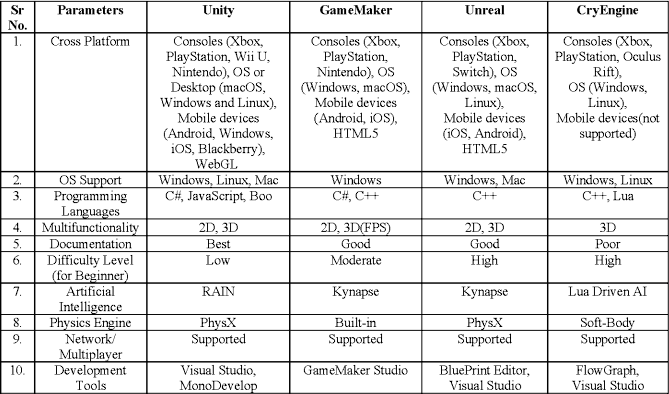
\includegraphics[width=0.9\textwidth]{images/GameEngineComparison.png}
    \caption{Game engine comparison, courtesy of \cite{9579618}}
    \label{image:gameEngineComparison}
\end{figure}
\pagebreak
\subsubsection{Graphics}
This is a big area of comparison between the two game engines, with Unreal engine being regarded very well in the industry for its very impressive graphics system due to its far more advanced rendering system compared to Unity that out of the box can produce much more impressive visual fidelity and finer looking results, however, this factor was not very important to me personally and as such, the increased graphical fidelity offered by the Unreal Engine was not a significant enough factor to affect my decision.
\subsubsection{Learning Value}
As the goal of the final year project is to further my own skills in software development according to my personal goals, one of the largest factors as regards choosing game engine was in fact the associated scripting language. I have a goal in the future to get a career in .net-based development and as such Unity's use of C\# was a major benefit for me in terms of learning the skills I desired to possess for my future career. And the fact that the C\# used in Unity isn't too dissimilar from standard C\# was a big bonus for me.
\section{Languages}
As mentioned earlier in the review language was a large factor in my choice for this project and the language that I intended to use was C\#. C\# is an object-oriented programming language developed by Microsoft which is used for developing desktop applications, games and web applications. It is frequently used to develop for Windows, iOS or Android. It is very heavily used in the software industry, according to a survey done by Stack Overflow in 2022, 29.7\% of developers claimed to use it \cite{stackOverflowSurvey2022}, meaning that it ranked as more popular than C and C++ in the same survey and less popular than Java.
\par
C\# is a strongly typed programming language, meaning that all variables must be declared with a specific type unless they are declared as either var or dynamic, variables specified as var will however still function as strongly typed and the type of variable is assigned at compilation based on how the variable is used. variables declared dynamic are instead resolved in run-time, however, I will not delve into these variables as I feel their use detracts from the advantage of a strongly typed language, that being that code is more readable and self-documenting, leaving less guesswork to the developer.
\par
As C\# is used with the .NET framework, it runs on the .NET Common Language Runtime which means that it avails of the CLR's built-in garbage collector. The presence of an in-built garbage collector ensures that I don't have to worry about the manual management of memory when writing code, it ensures that any unused objects will be cleared from memory avoiding memory leaks and improving the security of written code. The garbage collector works by checking if an object can be accessed through the application's code and if not, the memory used by the object is freed up, this behaviour can be modified using weak references, in that objects which can be accessed by code through a weak reference can still be collected using the garbage collector.
\subsubsection{Benefits of Object-Oriented Programming}
C\# is an object-oriented programming language, meaning that code is largely classed into classes and objects, this naturally complements game development very well as all the individual components making up a game can easily be thought of as objects, and the nature of object-oriented programming with each class containing its own associated data and methods makes it much easier to develop game components in a modular fashion and then integrate with each other.
\par
Additionally, aspects like encapsulation, meaning that the variables or properties that affect the internal state of an object can be isolated, meaning that we can ensure these instance variables that we wish to be private can only be accessed through the use of specific methods designed for classes. This makes the code more reliable and less bug-prone as it makes it easier to keep track of the different ways that objects can interact with one another.
\par
Other object-oriented principles such as polymorphism also make it easier to write more versatile code which can be modified in different ways depending on the particular goal, function overloading is the case that was most interesting to me, as with the purpose of the game being around evolution, there was the important aspect that the creatures in-game where e
\par
The object-oriented nature also made it easier to implement different performance-improving features that I figured would be necessary for the project, such as object pooling, which due to inheritance meant a generic object pool could be written to store any kind of game objects/
\section{Neural Networks}
In this chapter, I will be delving into Neural Networks which are an important aspect of my project. I will be writing a bit about them and several key aspects and justifying why in the end I chose to use a rather simple implementation of one.
\subsection{Introduction of Neural Networks}
Neural networks which at least in part were inspired by attempts at understanding the manner in which natural neurons operate and work in organic organisms. Neural networks are a broad class of machine-learning models which can be used to recognize patterns and create systems which can be trained to perform certain roles or tasks either using pre-obtained training data or through live feedback.
\par
Neural networks can be represented as directed graphs, and are most often composed of a variety of nodes or neurons which are linked together through connections which can have their own weights affecting the values of the outputs that they transmit.
The \ref{image:neuralNetworkStructure} provides a sample structure of a feed-forward neural network, meaning a network wherein there are no cycles formed by any looping connections between nodes. This sample structure is a neural network with an input layer, 2 hidden layers and an output layer.
\begin{figure}[ht!]
    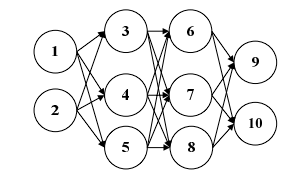
\includegraphics[width=0.9\textwidth]{images/NeuralNetworkStructure.png}
    \caption{Sample Structure of Feed-Forward Neural Network, courtesy of \cite{GURESEN2011426}}
    \label{image:neuralNetworkStructure}
\end{figure}
\par
I have included an image of a simple feed-forward neural network, as in the context of my project I intend only to include a small feed-forward neural network without even utilizing the advantages of more advanced training techniques like back-propagation as I feel that they don't fit in properly with the goals of my project.
\section{GitHub Copilot}
GitHub Copilot is an AI-powered coding assistant developed by a collaboration between GitHub and OpenAI. It is based on the Codex model developed by OpenAI \cite{OpenAICodex}, which itself was built upon the GPT-3 architecture. 
\subsection{Advantages of GitHub Copilot}
GitHub Copilot can offer developers intelligent suggestions as they type, anything from singles lines of code to entire blocks of code, which if using the Copilot extension in your IDE can simply be used with auto-complete, for example by using the tab key in Visual Studio.
\par
GitHub Copilot can also synthesize entire blocks of code or functions based on comments, taking the comments as suggestions and providing auto-complete suggestions that will meet the request.
\par
GitHub Copilot also displays an apparent ability to learn from context based on a user's project, with the suggestions becoming more accurate and appropriate to the work being done if the user engages with Copilot by accepting relevant suggestions and rejecting those that are inaccurate or irrelevant to the developer.
\par
An advantage of GitHub Copilot that was particularly relevant to me was that GitHub Copilot as of the time of writing this dissertation is available for free use by students, giving students an opportunity to get experience with GitHub Copilot for free so that we will likely grow accustomed to its use and continue to use in professional careers as software developers.
\section{Summary}
In Summary, I have decided that I will use Unity as my game engine for development, with C\# as the programming language of choice and that I will use a simple feed-forward neural network for controlling the creatures in my simulation.
\chapter{System Design}
This project was written entirely within Unity so in this section I will be dealing with the structure of the Unity game and I will go into how different aspects of the game work with explanations and references to relevant snippets of code or algorithms used.
\section{Scenes}
For SlimeWorld there are two scenes, the main menu which the player enters upon starting the application and the game scene in which the simulation occurs. The main menu contains, buttons to enter the main game, to quit the game and also to open the settings menu where the parameters of the simulation can be altered using a set of sliders.
\section{Menu Scene}
The menu scene is the simpler of the two scenes and it is responsible for giving the users the opportunity to change the settings of the simulation and to launch the simulation.  This image \ref{image:mainMenuHierarchy} shows the hierarchy of the scene in the Unity editor. As seen here there are two sets of menus, the "main" menu and the settings menu.
\begin{figure}[ht!]
    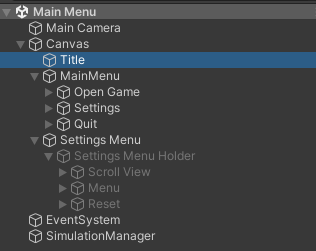
\includegraphics[width=0.5\textwidth]{images/MainMenuHierarchy.png}
    \caption{Main Menu Hierarchy}
    \label{image:mainMenuHierarchy}
\end{figure}

\subsubsection{Main Menu}
The main menu as seen here \ref{image:mainMenuPicture} is very simple containing the title of the game at the top of the screen and 3 buttons: Play, Settings and Quit. The play button sends the player into the Game scene, the Settings button opens the settings menu and the Quit button causes the game to close.
\begin{figure}[ht!]
    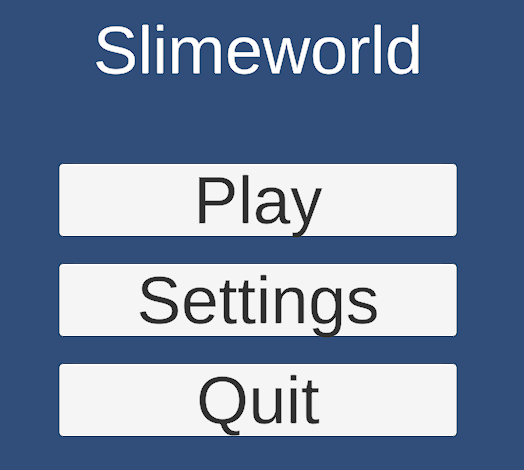
\includegraphics[width=0.5\textwidth]{images/MainMenuPicture.png}
    \caption{Picture of the Main Menu}
    \label{image:mainMenuPicture}
\end{figure}
\subsubsection{Settings Menu}
The settings menu as seen here \ref{image:settingsPicture} contains a scrollable view which contains the settings for the different parameters of the simulation, which are altered using the sliders. When the settings menu is opened, the SettingsMenu script gets all of the settings properties which are associated with the SimulationManager script and assigns them to the relevant sliders. When a slider is used, it calls the relevant method attached to slider, passing in its updated value and the updated value is in turn assigned to the relevant property of the SimulationManager and saved as a player preference. If the user clicks Menu the settings menu will be deactivated and the main menu will be reactivated. If the user clicks Reset, all playerprefs will be wiped, resetting settings to default values and also returning the player to the main menu.
\begin{figure}[ht!]
    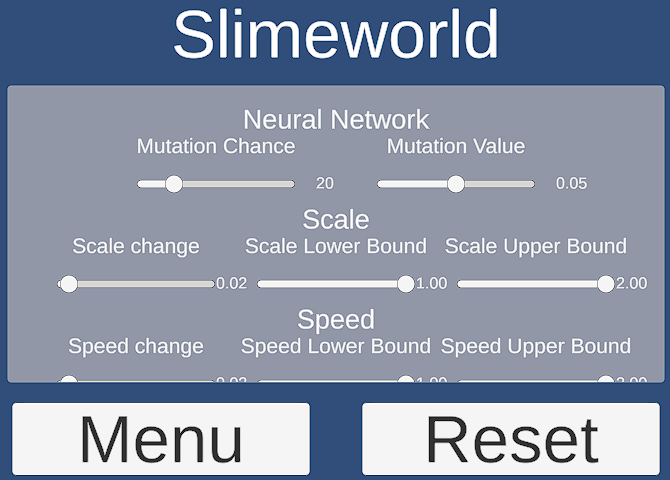
\includegraphics[width=0.5\textwidth]{images/SettingsPicture.png}
    \caption{Picture of the Settings Menu}
    \label{image:settingsPicture}
\end{figure}
\subsubsection{Simulation Manager}
The Simulation Manager is a singleton script which is shared across both the Menu and Game scenes, but I shall put it in the Menu scene as in normal usage of the application, the menu scene is where it is initialized. The SimulationManager script is responsible for loading and storing saved user settings and handling any modifications of the properties used to store them.
\par
The SimulationManager makes use of the singleton design principle to enable easier inter-script communication as access to its properties is required by many of the scripts in the game scene, including the SlimeManager script, FoodManager script and NeuralNetwork script.
\par
The SimulationManager makes heavy use of C\# properties to handle manipulation of settings and an example of one such property is found in this code snippet \ref{lst:cSharpProperty}. Where the properties of the property make it easy and convenient to handle modification of \_mutationChance variable and make it easy to determine when a property is modified.
\begin{lstlisting}[language=csh, caption=C\# Property, label={lst:cSharpProperty}]
    private int _mutationChance;
    public int MutationChance
    {
        get => _mutationChance;
        set
        {
            _mutationChance = value;
            PlayerPrefs.SetInt("MutationChance", value);
        }
    }
\end{lstlisting}
\section{Game Scene}
The Game scene is the main scene of the game and is responsible for the simulation of evolution by providing a small environment in which the slime can spawn and eat and reproduce or die. This image \ref{image:gameHierarchy} shows the hierarcy of the scene in the Unity editor.
\begin{figure}[ht!]
    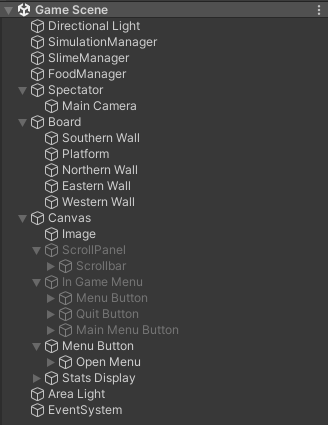
\includegraphics[width=0.5\textwidth]{images/GameSceneHierarchy.png}
    \caption{Game Hierarchy}
    \label{image:gameHierarchy}
\end{figure}
\subsection{Slime Manager}
The SlimeManager is a singleton script which is responsible for the spawning and disabling of slimes, upon entering the game scene or if the number of slimes dips too low, the SlimeManager will trigger a method called SpawnWave, which will spawn a number of slimes decided by the setting in the settings menu mentioned earlier.
\par
The SlimeManager is responsible for the spawning of slimes both with and without parent slimes, and to this end, the SlimeManager contains an instance of ObjectPool which stores slime GameObjects. When the SlimeManager spawns a slime it first must calculate the position of the new slime, which is a random position anywhere on the board if the slime is parent-less and is within 2 units on the x and the y axis of the parent if the slime has a parent. The SlimeManager then gets an instance of the slime GameObject from ObjectPool, assigns it a name which is Slime\_ followed by a number representing the number of slimes that had spawned before it. 
\par
For slimes without parents, the scale and speed values are determined randomly with regard to the lower and upper bounds for each value determined using the settings menu, a code snippet explaining this alongside the names is here \ref{lst:parentlessSlime}. 

\begin{lstlisting}[language=csh, caption=Parent-less Slime, label={lst:parentlessSlime}]
    spawnedSlime.name = string.Format("Slime_{0:00000}", _slimeCount++);
        Slime spawnedSlimeScript = spawnedSlime.GetComponent<Slime>();

        //float scale = UnityEngine.Random.Range(0.5f, 2f);
        //float speed = UnityEngine.Random.Range(0.5f, 2f);

        float scale = UnityEngine.Random.Range(SimulationManager.Instance().ScaleLowerBound, SimulationManager.Instance().ScaleUpperBound);
        float speed = UnityEngine.Random.Range(SimulationManager.Instance().SpeedLowerBound, SimulationManager.Instance().SpeedUpperBound);

        // pseudo constructor method for game object
        spawnedSlimeScript.Init(scale, speed);
\end{lstlisting}
\par
For slimes with parents, the method is much more complicated and takes the parent slime as a parameter. Seen here is the code \ref{lst:parentedSlime}, some of which has been removed for conciseness, but as can be seen, the child slime takes the parent's generation plus 1, receives a copy of their slimeInfo and a copy of their neural network.
\begin{lstlisting}[language=csh, caption=Slime with Parent, label={lst:parentedSlime}]
        // generation = parents generation + 1
        int generation = parentSlimeScript.GetGeneration() + 1;

        // parent's slime info is saved to be passed in to save variable
        SlimeInfo slimeInfo = parentSlimeScript.GetSlimeInfo();

        // parent's neural network is saved to be passed in
        NeuralNetwork neuralNetwork = parentSlimeScript.GetNeuralNetwork();

        // As it is unwise to create instance of classes extending monobehaviours using the new command, the init command is used as a pseudo constructor after the gameobject has been instantiated
        spawnedSlimeScript.Init(scale, speed, generation, slimeInfo, neuralNetwork);
\end{lstlisting}
\par
The last responsibility of the SlimeManager as mentioned earlier is to deactivate slimes when they've either been eaten or rotted away and to this, the SlimeManager simply calls the DeactivateObject method on the slime in question, returning it to the object pool.
\subsection{Slime}
The Slime is the most important class in the scene and game, as it represents the creatures which are being evolved in the simulation. The slimes have a number of persistent variables associated with them, their scale and speed which are floats, their generation which is an int, alongside their slimeInfo which is a SlimeInfo and their neuralNetwork which is a NeuralNetwork. All of these are inherited from a parent if said parent exists.
\par
The slime's scale represents its size and if a slime is 10\% larger than a smaller slime, it can eat the slime upon collision and convert it to saturation, which is a measure of the number of calories the slime has. The slime's speed represents its movement speed. Both scale and speed have a metabolic cost in the simulation with slimes with higher numbers in either trait having a proportionally higher energy upkeep.
\par
The SlimeInfo is a simple class used to store a slime's name, scale, speed, generation and number of children alongside the instance of its parent SlimeInfo, this is used to create a sort of linked-list of slimeInfos which can be used to keep track of the ancestry of slimes. Here is a code snippet \ref{lst:parentedSlimeInfo}, which contains the constructor for SlimeInfo when a slime has a parent.
\begin{lstlisting}[language=csh, caption=Slime Info with Parent, label={lst:parentedSlimeInfo}]
        // Constructor for slime with parent, takes the generation and parentSlime as additional paramters
    public SlimeInfo(string slimeName, float slimeSize, float slimeSpeed, int slimeGeneration, SlimeInfo parentSlime)
    {
        SlimeName = slimeName;
        SlimeScale = slimeSize;
        SlimeSpeed = slimeSpeed;
        SlimeGeneration = slimeGeneration;
        // The SlimeInfo parentSlime is a way to set the connect the parentSlimeInfo to this slimeInfo approximating a linked list
        ParentSlime = parentSlime;
        SlimeChildren = 0;
    }
\end{lstlisting}
\par
The slimes behaviours are controlled by a neural network which is a mutated copy of their parent's neural network, though the mechanics of this will be analyzed more in-depth in the Neural Network section.
\subsection{Neural Network}
The Neural Network implemented in SlimeWorld is a simple neural network which does not make any use of back-propagation or other more advanced training techniques, the reason for this is that in order to more accurately approximate evolution, the neural network has no scoring parameters for evaluating its performance, and with the sandbox nature of the simulation it would be rather awkward to try and set any parameters by which to measure the success of the neural network. 
\par
To this end, the neural network is one of the simplest variants, with the modifications being an unmodified random chance, which is applied equally to every weight and bias in the network. The downsides of this approach are obvious in that the neural network will neither be trained quickly nor to a high degree of accuracy.

\subsubsection{Inputs and Outputs}
For the neural network, one decision I made early on was that I wanted to ensure that every input was normalized to be within the same range, this was a design decision that I could implement without too much difficulty as all inputs would be generated by the slimes in-game. As I had settled on tanh as my activation function, I decided to keep all inputs and outputs of the neural network between -1 and 1.
\par
The topology of the neural network that I have used for this project is 12 nodes in the inputs layer, 8 nodes in the first hidden layer, 5 nodes in the second hidden layer, and 2 output nodes. I have classified the input nodes into three sections based on what kind of information they contribute to the neural network, the first being internal information \ref{lst:neuralNetworkThisSlime}, being information that pertains to the slime itself and contains 3 input nodes.
\begin{lstlisting}[language=csh, caption=Neural Networks inputs for The Slime, label={lst:neuralNetworkThisSlime}]
    // Represents slimes current hunger, updates every in-game update
    _inputsToNeural[0] = _saturation / 50f - 1f;

    // Setting neural inputs that persist for the life of the slime, as neither _scale nor _speed can change, these inputs are set once and never changed
    _inputsToNeural[1] = _scale;
    _inputsToNeural[2] = _speed;
\end{lstlisting}
\par
The next category of information for the slime is that related to food which contains 3 input nodes \ref{lst:neuralNetworkFood}. and the final category of information being that related to other slimes which contain 6 input nodes \ref{lst:neuralNetworkOtherSlimes}.
\begin{lstlisting}[language=csh, caption=Neural Networks inputs for Food, label={lst:neuralNetworkFood}]
     // Represents saturation of food, -0.5f due to following formula
    // value = (saturation / 50) - 1, so for food which has default 25 = -0.5f
    _inputsToNeural[3] = -0.5f;
    // Represents angle of food relative to slime in pi radians to fit in with scheme of inputs being -1 to 1,
    // Negative values are on the left side, positive values are on the right
    _inputsToNeural[4] = (Mathf.Deg2Rad * Vector2.Angle(transform.forward, (Vector2)(_closestFood.transform.position - transform.position))) - 1;
    // Represents distance to food from slime, with values between -1 and 1,
    // And distance greater than 25 is capped at an input value of 1
    _inputsToNeural[5] = Mathf.Clamp((Vector3.Distance(_closestFood.transform.position, transform.position) / 12.5f) - 1f, -1f, 1f);
\end{lstlisting}
\begin{lstlisting}[language=csh, caption=Neural Networks inputs for other slime, label={lst:neuralNetworkOtherSlimes}]
    Slime closestSlimeScript =
    _closestSlime.GetComponent<Slime>();
    // Represents scale of closestSlime, values are clamped between 0.5 and 2 typically
    // So take away one to fit within established scheme for neural net inputs
    _inputsToNeural[6] = closestSlimeScript.GetScale() - 1;
    // Represents speed of closestSlime, values are clamped between 0.5 and 2 typically
    // So take away one to fit within established scheme for neural net inputs
    _inputsToNeural[7] = closestSlimeScript.GetSpeed() - 1;
    // Represents angle of closestSlime relative to slime in pi radians to fit in with scheme of inputs being -1 to 1,
    // Negative values are on the left side, positive values are on the right
    _inputsToNeural[8] = (Mathf.Deg2Rad * Vector2.Angle(transform.forward, (Vector2)(_closestSlime.transform.position - transform.position))) - 1;
    // Represents distance to closestSlime from slime, with values between -1 and 1,
    // And distance greater than 25 is capped at an input value of 1
    _inputsToNeural[9] = Mathf.Clamp((Vector3.Distance(_closestFood.transform.position, transform.position) / 12.5f) - 1f, -1f, 1f);
    // Represents saturation value of closestSlime, calculated with following formula,
    // input = (saturationIfEaten / 50) = 1
    _inputsToNeural[10] = (closestSlimeScript.GetSaturationIfEaten() / 50f) - 1;
    // Represents status of closestSlime, 0 if dead, 1 if alive
    _inputsToNeural[11] = closestSlimeScript.IsAlive() ? 1 : 0;
\end{lstlisting}
\par
The training of the neural network is performed with a very naive and inefficient method, where when a NetworkNetwork is cloned from another, each bias and weight has a chance of changing a given amount based on the input parameters, which are set in the settings menu mentioned earlier.
\subsection{Food Manager}
The FoodManager script is a singleton responsible for the creation and removal of food in the simulation. The FoodManager has an ObjectPool instance containing a prefab for a food GameObject. Upon starting the game and every 10 seconds thereafter a specified amount of food, determined by the foodPerInterval setting is spawned unless the foodCap is reached at which point no more food will spawn until the food dips below the cap. When food is spawned, a food GameObject is pulled from the objectPool and placed at a random location on the map. And when a piece of food is eaten, it calls the FoodManager's DeactivateFood method which in turn calls the ObjectPool's DeactivateObject method.
\subsection{Object Pool}
I created my own implementation of an object pool as I felt that the object pool incorporated in Unity didn't properly satisfy my requirements. One of the key reasons was that I desired the ability to keep track of all active objects in the pool so that I could more easily perform checks to determine which entities were closest to one another by iterating through every entity on the list of active objects.
\par
The object pool is composed of list of GameObjects containing the active objects in game and a queue of GameObjects representing all the deactivated objects in the game. I picked a list to represent the active objects as I wished to be able to iterate through the list easily, while I felt that a queue would suit the inactive objects better, as all that was necessary was to store objects that were deactivated and then pop them from the front of the queue once a new object was needed.
\par
To make use of the object pool, I created a constructor which would take in the gameObject representing the prefab to be stored as a parameter as can be seen in this listing \ref{lst:ObjectPool}. I then made use of the object pools to store prefabs of both the foods and the slimes as both are frequently created and destroyed in the simulation.
\begin{lstlisting}[language=csh, caption=Object pool, label={lst:ObjectPool}]
    public ObjectPool(GameObject pooledObject)
    {
        _activeObjectPool = new List<GameObject>();
        _inactiveObjectPool = new Queue<GameObject>();
        _pooledObject = pooledObject;
    }
\end{lstlisting}
\par
After making the object pool, I had to make methods to use the object pool to provide objects when necessary which can be seen in this code snippet \ref{lst:ObjectPoolActivateDeactivate}. The purpose of the DeactivateObject method was to take in objects that were to be deactivated, set them to inactive, remove them from the list of active objects and then add them to the queue of inactive objects. The GetPooledObject method would check if the queue of inactive objects was empty and if so it would instantiate a new object based on the stored prefab, otherwise it would pop the deactivated object at the head of the queue and activate it, before returning it.
\begin{lstlisting}[language=csh, caption = Object pool activate and deactivate, label={lst:ObjectPoolActivateDeactivate}]
// Passed in object is deactivated, removed from the activepool and added to inactivepool
    public void DeactivateObject(GameObject objectToDeactivate)
    {
        objectToDeactivate.SetActive(false);
        _activeObjectPool.Remove(objectToDeactivate);
        _inactiveObjectPool.Enqueue(objectToDeactivate);
    }

    // Either returns an object from the inactiveObjectPool or instantiates a new object if the inactiveObjectPool is empty
    public GameObject GetPooledObject()
    {
        // Object variable is declared
        GameObject objectToReturn;
        if (_inactiveObjectPool.Count != 0)
        {
            // if inactivePool isn't empty then take object from queue
            objectToReturn = _inactiveObjectPool.Dequeue();
            objectToReturn.SetActive(true);
        }
        else
        {
            // if pool is empty then instatiate new object
            objectToReturn = Object.Instantiate(_pooledObject);
        }
        // object is added to activeObjectPool
        _activeObjectPool.Add(objectToReturn);
        return objectToReturn;
    }
\end{lstlisting}
\section{Spectator}
The spectator represents the user's camera and is a flying object which is controlled using WASD, E and Q for movement forwards, left, back and right and up and down. The Spectator uses the mouse for rotation, though if the escape is pressed, the cursor is unlocked so that it can interface with the UI. If the left mouse button is clicked while the user is moused over a slime, the statistics relevant to the slime and their ancestry is displayed \ref{image:inGameUI}.
\begin{figure}[ht!]
    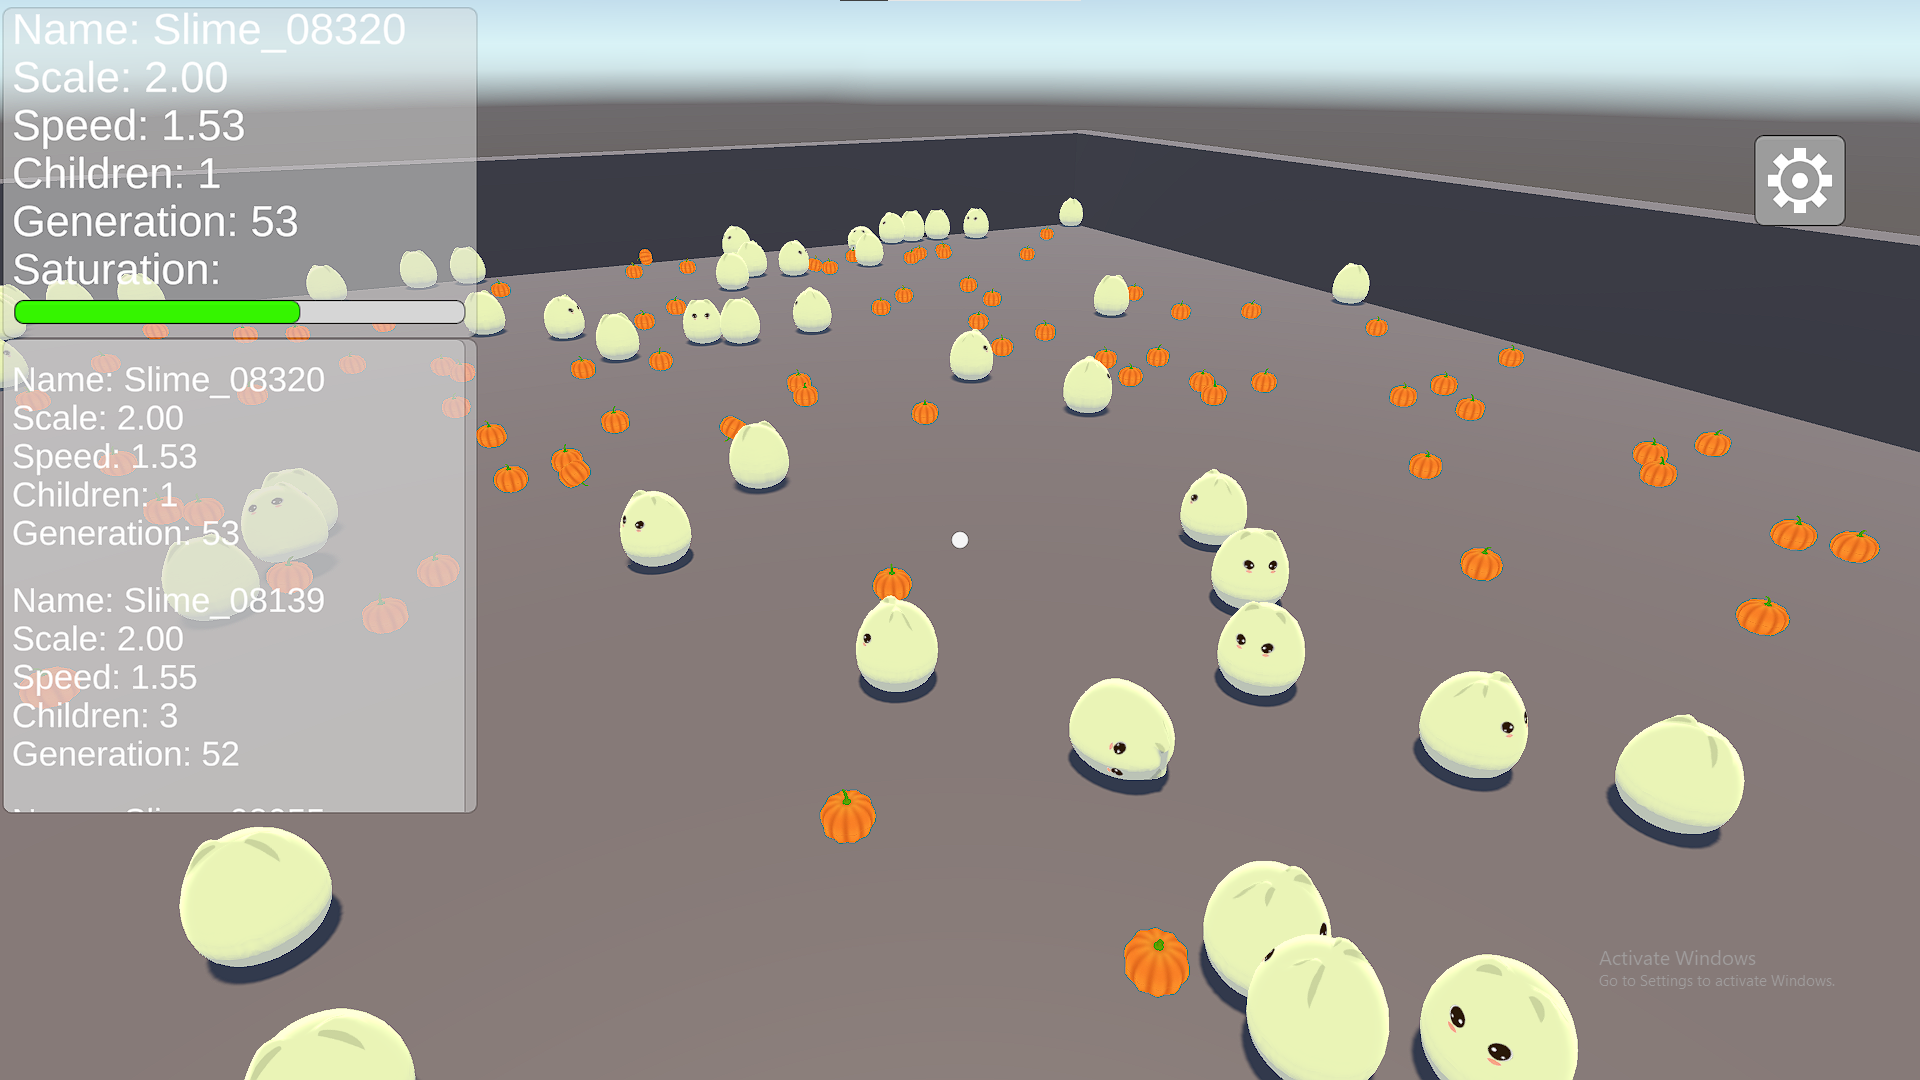
\includegraphics[width=0.5\textwidth]{images/GameUI.png}
    \caption{In-Game UI}
    \label{image:inGameUI}
\end{figure}
\par
The ancestry data, being populated using the slime's slimeInfo, and the attached reference to the previous generation's slime info, to iterate through them all and generate a list. Which is then assigned to a scroll-able list on the left side of the screen.
\par
if the user's mouse is unlocked and they click on the gear on the right side of the screen they open the in-game menu from which they have buttons to return to the main menu, quit the game outright or close the in-game menu \ref{image:inGameMenu}.
\begin{figure}[ht!]
    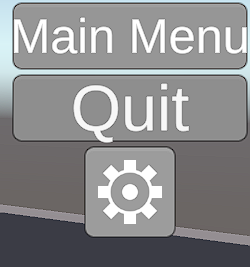
\includegraphics[width=0.5\textwidth]{images/Game Menu.png}
    \caption{In-Game Menu}
    \label{image:inGameMenu}
\end{figure}
\chapter{System Evaluation}
\section{Creating a 2d Plane for Simulated Life}
This was the easiest of the goals that I set out to do with my project and though it is an environment free of flair or any complexity I do feel that the project has succeeded in creating a simple environment which contains simulated life.
\section{Populating the Plane with creatures}
I feel that though life in the context of the simulation is rather simple, I do think that it satisfies my initial goals as life is capable of evolution albeit in a simple manner and only governing a few traits, and I am happy with the fact the creatures can both eat, starve and be eaten. I am also happy with the manner in which the creatures can reproduce and the fact that many of a parent's traits are successfully passed down to their offspring which small changes occurring as required to manifest evolution.
\section{To include a System for Creatures to Evolve}
I feel that this is an area where I had fallen short of my desired goals as I had originally wished to implement a greater variety of inheritable traits that could affect the creature's lifestyles and had hoped to do this through a more complicated system based on specific genes that might be passed down, though I thought this, in the end, unnecessary as it was excessive to model in a simulation with asexual rather than sexual reproduction.
\section{To have Creatures controlled by a Neural Network}
I feel that this was the greatest failure of the project as I feel that my approach of using a small feed-forward neural network didn't provide enough potential for the creatures to learn to display intelligent behaviour in regards to trying to stay alive and that the lack of a specialized training method due to the desire to avoid any inherent motivations in the system meant that the neural network would either train far too slowly or always overshoot the "optimal" weights and biases for its purposes.
\section{To support multiple "species" of Creatures, suited to different niches}
I feel that my project failed in reaching this goal due to shortcomings of the neural network and the shallowness of the traits I implemented which meant that there wasn't enough depth in the simulation for any sort of ecological niches to form, and to be filled, furthermore, I couldn't develop an algorithm which would be able to define species in the context of the simulation.
\section{To create a Tweakable Environment}
Though I pursued it in a simple manner I am happy with the fact that many of the aspects of the simulation can be modified by changing the settings of the simulation, leading me to believe that the environment is at least somewhat tweakable.
\chapter{Conclusion}
\section{Overview}
This section is where I'll summarize the goals of my project and how I feel my project performed as regards meeting them, I will also discuss what I think was the biggest flaw in my project as regards approaching these goals.
\section{Goals}
\begin{itemize}
    \item To create a 2d plane for simulated life to live on.
    \par
    I feel that this goal was met satisfactorily.
    \item To populate the plane with creatures which can eat, starve and procreate.
    \par
    I feel that this goal was met satisfactorily.
    \item To include a system for the creatures to evolve throughout generations, passing traits along to their children.
    \par
    I believe that this goal was achieved though not with the same level of depth as I'd desired.
    \item To have the creatures controlled by neural networks which themselves are also honed through this evolutionary process.
    \par
    I believe the neural networks are the largest failure of the project so I will detail why further on in this chapter.
    \item To support multiple "species" of creatures, suited to different evolutionary niches
    \par
    I believe that I have failed to achieve this goal as the environment created by the application was insufficiently complicated to provide ecological niches for slimes to shape themselves to and the slimes themselves were insufficiently intelligent.
    \item To create a tweakable environment which can affect the evolution of the creatures.
    \par
    Though the end implementation of tweakable settings for governing the environment was done rather simply, I do feel that the settings as they are, work reasonably well within the system and I considered the goal satisfied.
\end{itemize}
\section{Faults with the Neural Network}
\subsection{Inefficient Training Methodology}
A big aspect of the inefficiency was the intentionally simplistic model in which the neural networks were trained, as utilizing more efficient methods like back-propagation in the training of the neural networks would have detracted from the goal of modelling evolution, by necessitating specific scorable criteria for the slimes which would need to be used to evaluate their relative fitness and hence the degree of change which should be made in the neural network.
\par
As while the training method implemented in the system is currently a very naive training method, which doesn't take anything into account regarding the performance of the neural network, I couldn't come up with a better method for training neural networks which didn't include any scorable or defined goals which would be used to measure it's performance.
\subsection{Rigid nature of Neural Network}
However, what I think was actually the larger shortcoming of the neural network was that despite the free-form nature of neural networks in that the ways they process data are undeniable but the main issue was actually with the rigid nature of the inputs. The inputs of the neural network govern its potential alongside a greatly increased training period with a larger amount of input nodes. 
\par
The manner in which this issue has manifested in the project has actually been in regard to how the slimes track other entities, for as is seen in this code snippet \ref{lst:neuralNetworkOtherSlimes}, half of the neural network's inputs are dedicated to observing the information of just one other slime. And the most crucial downfall of this, is that no matter how refined the neural network would become, through potentially millions of cycles of training, it could never properly learn to tackle situations with multiple competing slimes as the slime can only ever perceive one other slime at a time.
\par
This is a fundamental issue with the neural network as I see no manner in which to attempt to solve the issue while keeping any aspects of the neural network as it is currently outside of retaining the 2 output nodes. Because should the developer decide to tackle this issue by providing additional sets of input nodes to handle more slimes, it will risk drowning out the other inputs of the neural network, and the number of slimes that could be tracked would still be rigidly defined by the size of the inputs.
\par
In Summary, the issue regarding the rigid nature of the neural network is that at least in the implementation that I have gone with, there is no way in which the input systems can be modified to work with a dynamic number of entities. Hence if I were to tackle this project again, the main differences I would make would be in regards to the topology of the neural network and performing far more research into the different forms of neural network or machine learning systems which can be made to more easily work alongside systems such as arrays or other lists of inputs.
\include{appendices}



%------------------------------------------------------------------------------------------------------	
% Generate the bibliography. You may have to build the document more than once before all of the
% references and processed and cited correctly.
% WARNING: Don't mess with any of the following unless you know what you are doing.
%------------------------------------------------------------------------------------------------------	
\bibliographystyle{unsrt}
\bibliography{references.bib}
\end{document}